\documentclass[a4paper,12pt]{article}
\usepackage[utf8]{inputenc}
\usepackage{graphicx}
\usepackage{float}
\usepackage{parskip}
\usepackage[style=apa]{biblatex}
\addbibresource{exp.bib}

\title{TOK: What challenges are raised by the dissemination and/or communication of knowledge?}
\author{Terry Qi}

\begin{document}

\maketitle
\begin{enumerate}
 \item The law of demand in my Economics book
 \item The bible according to Spike Milligan
 \item My Firefox progress bar
\end{enumerate}

\newpage

% breakdown of
% theme of does empirical evidence impiy knowledge in the sciences. question
% LOD: social sciences, hypothesize, trend
% double pendulum: the natural sciences, chaotic application, predicable path, yet no knowledge of its location
% progress bar: provenable knowable yet pretend to be in control. questions the motivation to certainty,


% intro
The TOK prompt I have chosen is: ``What challenges are raised by the dissemination and/or communication of knowledge?''. This exhibition will explore the prompt by reflecting upon knowledge within the sciences, more specifically answering whether uncertainty hinder the acceptance and communication of knowledge. While mathematicians often take deductive proofs as granted, this is less common in the area of sciences. Every experiment contains empirical results, but depending on different people with their own personal backgrounds, beliefs, ideologies, or perspectives, the significance of the result will differ between the public. More directly, the lack of trust in the sciences may be a disbelief towards its empirical methods, that uncertainty is untrustworthy and does not bring knowledge.


% knowable thing but could be failified
\subsection*{Object \ref{fig:lod}, The Law of Demand}

\begin{figure}[h!]
 \centering
 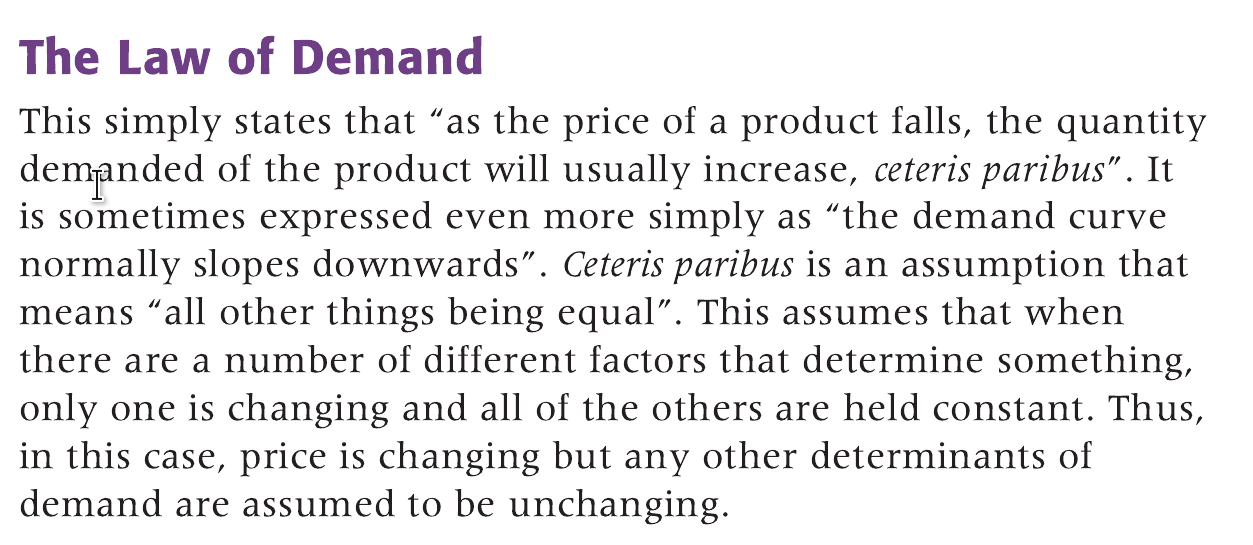
\includegraphics[scale=0.3]{ecobook.png}
 \caption{The law of demand in the book}
 \label{fig:lod}
\end{figure}

This formula comes from my economics course book, and serves to be a controversial topic for its inclusion of the word ``law'', with the formula being the historical avant-garde of a sense of certainty within the social sciences. The idea is however attacked frequently, particularly by psychologists arguing that the law is too idealistic in the context of real life, therefore creating a new branch of economics --- behavior economics \parencite{DKahneman}.

The equation is interesting for it is an expression of the bold beliefs of scientist in their models. Economists often back up the law through unrealistic claims that are intentionally broad, marking its failures as a violation of the ``axioms'' of standard economic theory and the case should be treated separately. This showcase a case of false certainty --- marking a relationship of human behavior to be more knowable than it truly is. On the one hand, it justifies many aspects of modern economic theories, with empirical proof of the success reflected in economical growth number; but it also creates confusions for the learners and critics: coming from a maths background, I did not initial buy into the ``law'' for its vagueness. The framework allows economists to justify their actions while leaving the interpretation of their building blocks to be broad and uncritiqueable.

This object reinforces the difficulties and consequences when uncertain events are framed to be certain. The natural scientists' critique only serves to reveal the flaws in their ``scientific methods'', that the entirety of physics is in essence, fitting numbers to interpretations. While both parties disagrees in acknowledging the shakiness of their disciplines, they are similar in framing the confusion as an ``interesting property'' and a benefit of the sciences, ultimately displaying how the interpretation of empirical evidence differs depending on your personal beliefs and backgrounds.

% knowable thing but is chaotic
\subsection*{Object \ref{fig:bible}, The bible according to Spike Milligan}

\begin{figure}[h!]
 \centering
 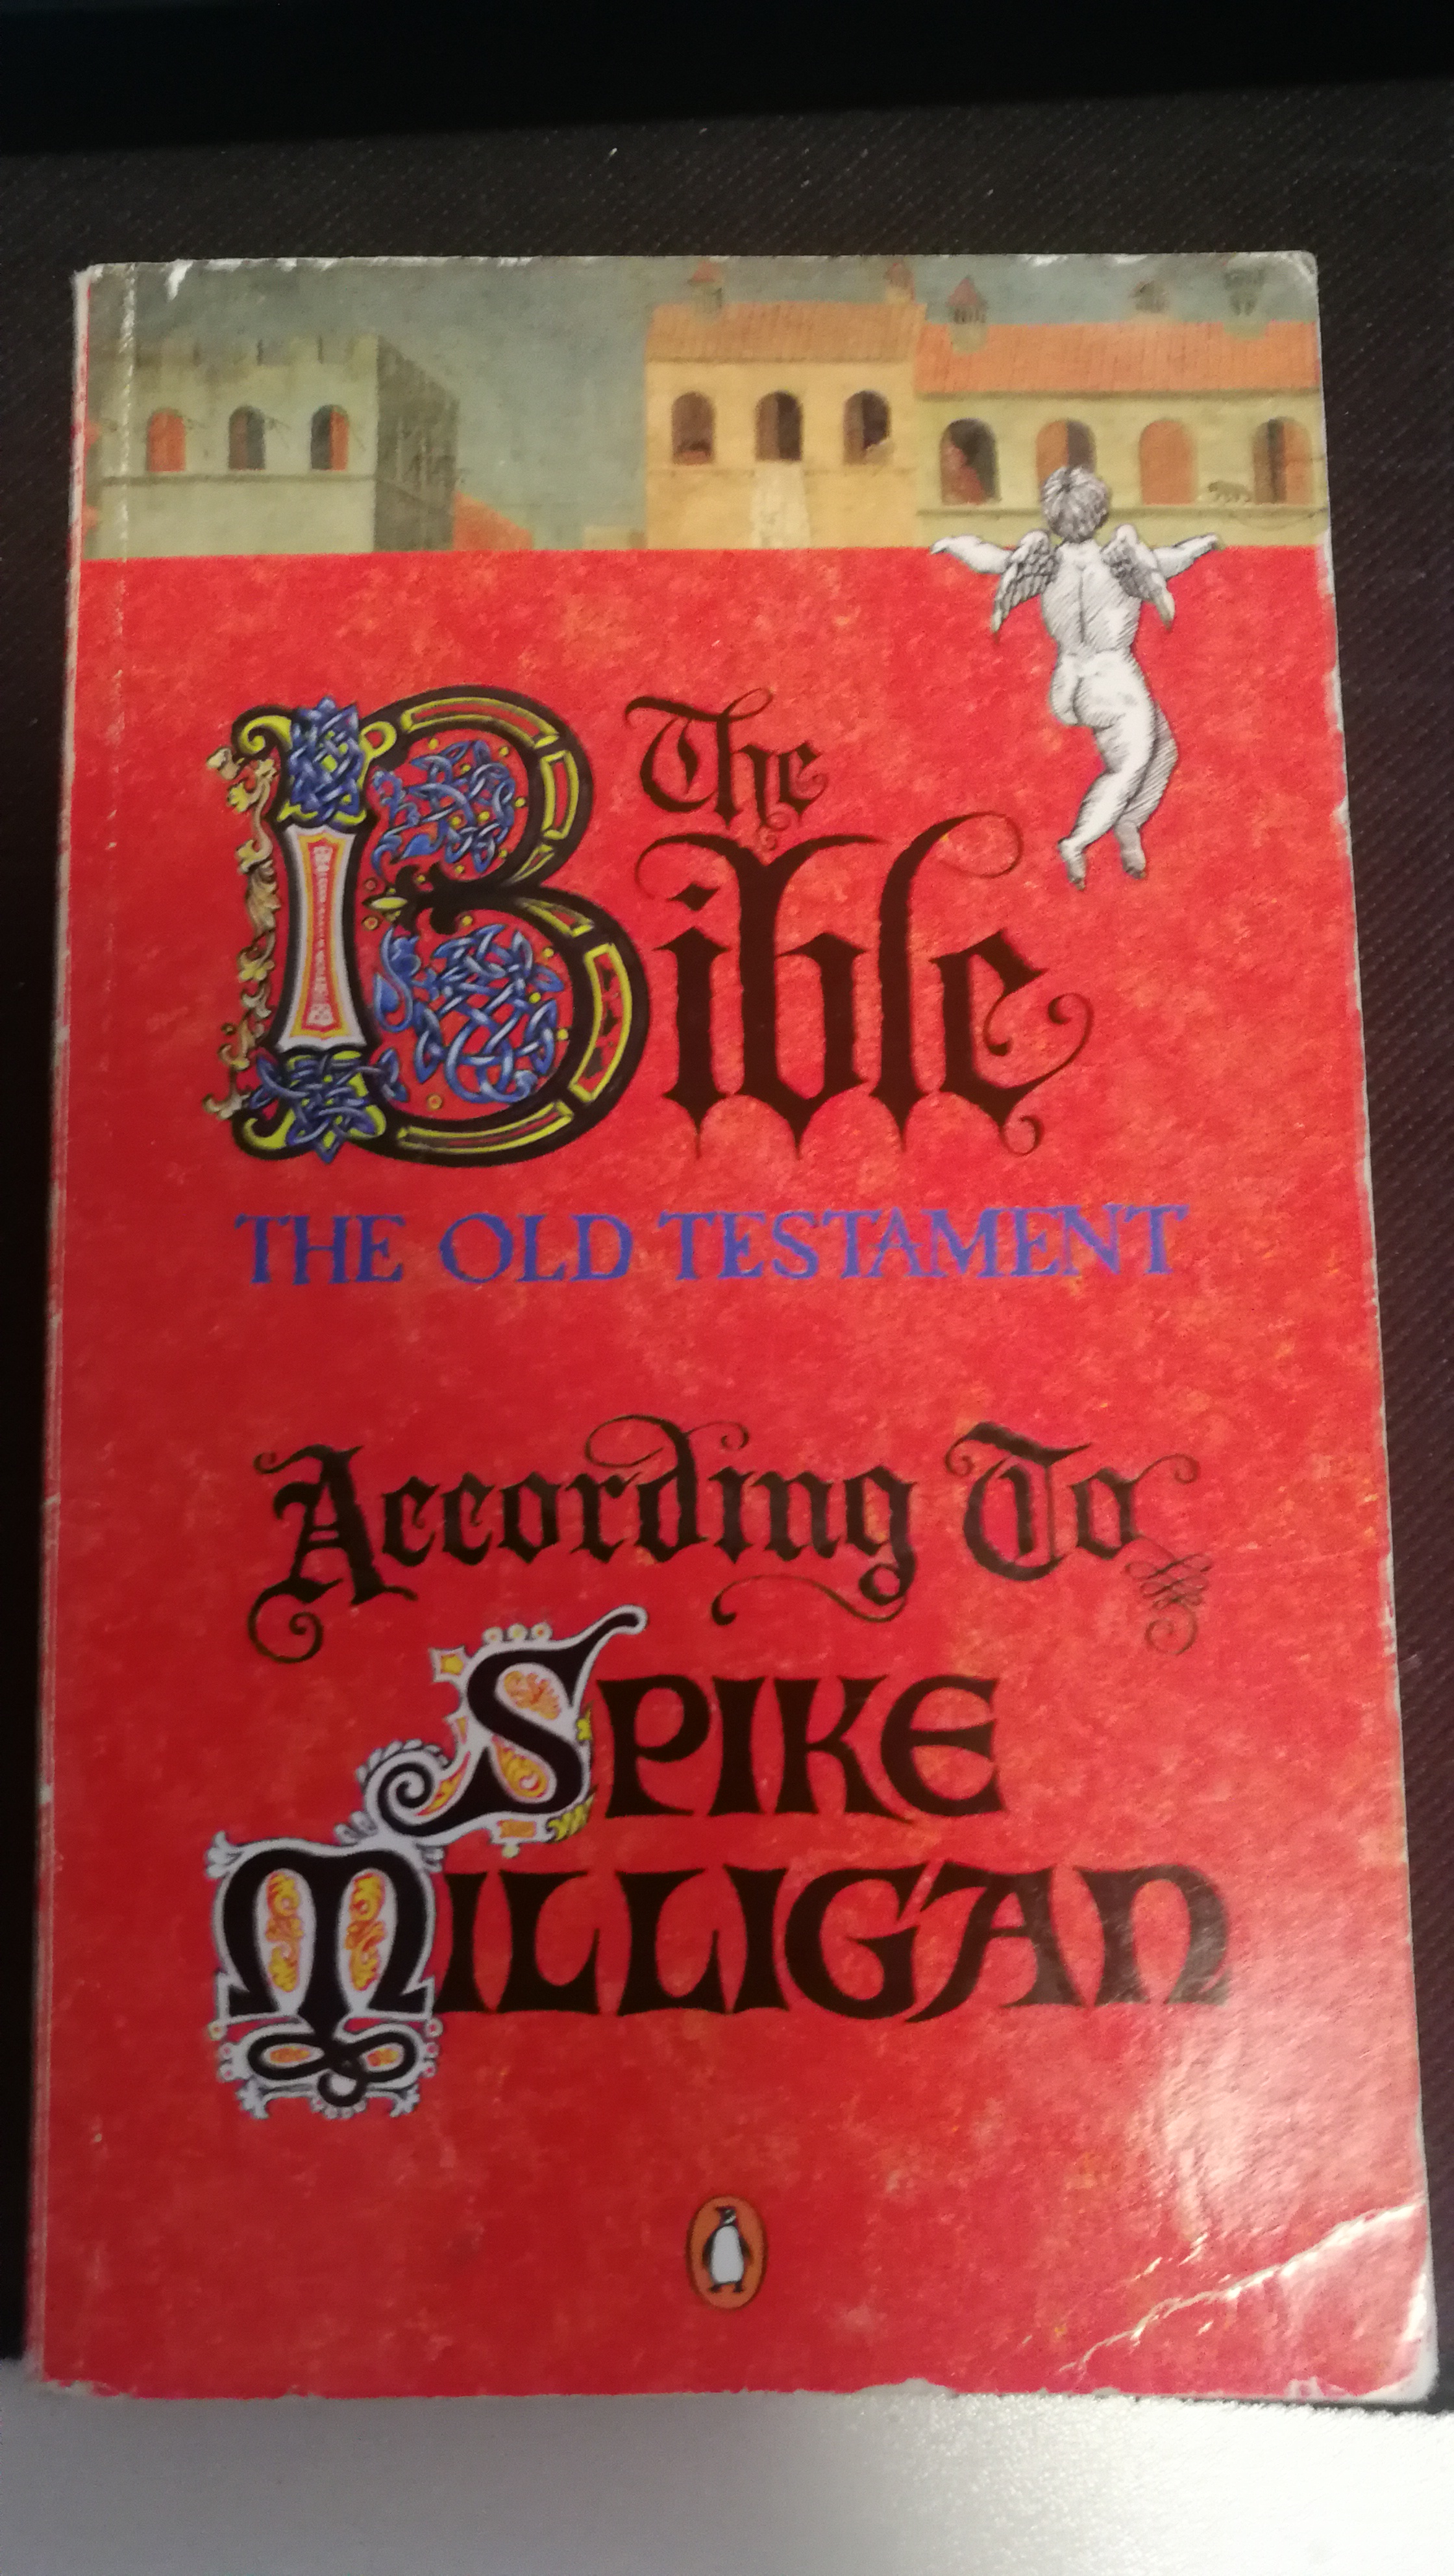
\includegraphics[scale=0.1]{bible.jpg}
 \caption{The bible according to Spike Milligan}
 \label{fig:bible}
\end{figure}

The object is a book issued to me by my history friend out of interest, for it parodies the old testament section of the bible. When people think about the bible, they think of the connection and quotations within it rather than the plausibility and validity of the work. Historically speaking, the bible is special in its unknown origin and writer. Some people view this uncertainty as an argument to reject all meanings within the book, some accepts the knowledge it presents and not by its origin, and some values both interpretations equality.


The parody of the bible is intriguing for it beautifully shows how the context of its origin can be completely different while retaining its messages and knowledge. The first chapter references the creation of the world, but from a perspective of a British startup firm. Unexpectedly, this shows that the messages of the bible --- that God is took seven days to create the world, is independent of its context, showcasing how the uncertainty of the origin can have little effects on the knowledge presented.

Therefore I have included this bible in the exhibition to be an example where the uncertainty fails to hinder the communication of underlying values. Judging from the positive reviews from the various purchasers and I, it seems to display the ability of a common ideology or pure interest to decrease the significance of the context of knowledge. This is in analogy to the ideas presented by the economists --- that the idealistic axioms are justified by a significant result in the knowledge that it creates.


% The object is my personal simulation of some swinging double pendulums. On the surface, it seems that the advances in the natural sciences should be able predict its motions to the atom. But the discovery of chaos questions the fundamental values of physics as a whole. In a sense, some people consider the possibility of uncertainty to be roadblock in the acquiring of knowledge in the sciences.

%Physics as a discipline follows a trend of experiment, theories, and prediction to formulate our understanding of the universe.

% unknowable thing that expresses certainty
\subsection*{Object \ref{fig:download}, The Firefox Progress bar}

\begin{figure}[h!]
 \centering
 
\includegraphics[scale=0.35]{progress.png}
 \caption{The Firefox progress bar}
 \label{fig:download}
\end{figure}


The object is a progress bar of a file download in the my Firefox browser. It have the purpose of displaying the time it takes to download this very important file I need. This sight had only became more common in the information era, yet it had surprised me to know that the underlying progress it displays has no certainty. The progress bar serves as a distraction to the nondeterministic information of file downloading for the user.

While this little bar can come in many forms, there exist an endless flow of people complaining the inaccuracy of the device, yet the purpose of the device is for good --- to create feedback upon an action. It implies the idea that covering uncertainty with certainty, where knowledge is deliberately hidden, is undesirable to people. Additionally, versions of progress bars which does not cover the uncertainty does not escape the criticisms. It seems to me that people fear the concept of covering uncertainty with certainty, showcasing inability to reduce uncertainty in the communication of knowledge.

The common appearances (and criticisms it faces) of the item helps in broadening the scope of the knowledge question. The progress bar showcases the general knower's desire for information in the event of a knowledge barrier, and its fear for the censoring of knowledge. For I have made progress bars myself in my apps, I find the understanding of the underlying knowledge the bar covers --- whether uncertain or not, helps in reducing the frustration of such a progress bar. This showcases the ability of uncertainty, even if covered with certainty, to induce frustration and communication of knowledge.


\newpage
\nocite{*}
\printbibliography


\end{document}
